\documentclass[11pt,a4paper]{article}

\usepackage{array}
\usepackage{float}
\usepackage{graphicx}
\usepackage{tabularx}

\usepackage[section]{placeins}
\usepackage[margin=1.0in]{geometry}

\begin{document}
\title{BatSignal:\\System Design Document}
\author{
	Joe Moraal\\moraalj@wit.edu\\ \and
	Zach Thornton\\thorntonz@wit.edu \and
    Bryan Young\\youngb2@wit.edu \and
	Computer Science 2015 \\
	Wentworth Institute of Technology
}
\date{\today}

\maketitle
\newpage

\tableofcontents{}
\newpage


\section{Introduction}

\subsection{Purpose and Scope}
This document describes the hardware and software components of the BatSignal distributed sensor network. This document is intended for use by developers implementing BatSignal.

\subsection{Project Executive Summary}
% This section provides a description of the project from a management perspective and an overview of the framework within which the conceptual system design was prepared.  If appropriate, include the information discussed in the subsequent sections in the summary.
The system is designed as a rapid response alert system capable of identifying emergencies and reporting their location. The system passively captures audio from the sensors and analyzes it for keywords or phrases. When the system detects a match it dispatches an email to a list of administrators and displays a notification on the administration console. \\\\
The system is designed to be scalable according to the needs of the location of installation. Controller nodes are installed at or near administrative areas with sensor nodes installed in patient rooms, inhabited spaces, common areas, etc. Messages propagate through the BatSignal mesh network allowing nodes to communicate with the controller node despite the often significant distance between them.

\subsubsection{System Overview}
% This section describes the system in narrative form using non-technical terms.  It should provide a high-level system architecture diagram showing a subsystem breakout of the system, if applicable.  The high-level system architecture or subsystem diagrams should, if applicable, show interfaces to external systems.  Supply a high-level context diagram for the system and subsystems, if applicable.  Refer to the requirements trace ability matrix (RTM) in the Functional Requirements Document (FRD), to identify the allocation of the functional requirements into this design document.
The system is divided into two types of nodes.  These nodes form a mesh network that relays data from the first type of node, called sensor nodes, to the second type of node, called the controller node. \\\\
Python modules installed on the sensor nodes passively read input from a microphone. The input from the microphone is fed into Python's speech recognition module. The audio input is then sent to the controller node over the mesh network as JSON. \\\\
Python modules installed on the controller node passively receive the sensor's data.  It then parses through the text looking for alert phrases.  Upon recognizing an alert phrase an email is sent to a list of administrators containing the plain-text of the audio capture and the identifier for the sensor node that captured it.
\begin{figure}[H]
	\centering
		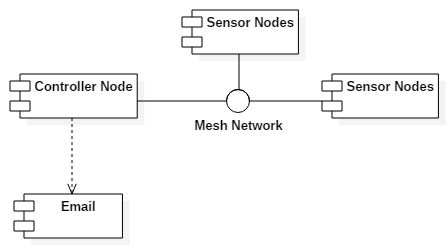
\includegraphics[scale=0.75, keepaspectratio=true]{Graphics/SimpleOverview.png}
	\caption{BatSignal system overview}
\end{figure}

\subsubsection{Design Constraints}
% This section describes any constraints in the system design (reference any trade-off analyses conducted such, as resource use versus productivity, or conflicts with other systems) and includes any assumptions made by the project team in developing the system design.
The BatSignal distributed sensor network will consist of numerous Raspberry Pi boards distributed across a physical area. This network has many constraints that must be considered. These constraints are as follows:
\begin{itemize}
	\item{\textbf{Maximum Node Separation Distance -}}
		The nodes must be close enough to communicate effectively with one another in order to form a reliable mesh network. This maximum effective communication distance relies on the capabilities of the Wi-Pi WLAN module and the B.A.T.M.A.N. routing protocol. This distance has not been determined yet. \\\\
		The communication range is also affected by physical objects in the installation environment, which may reduce the base measurement during implementation.
	\item{\textbf{Sensor per Controller Ratio -}}
		Due to the physical limitations of the controller node's processing power and each Wi-Pi WLAN module's transmission rate, coupled with the mesh network's maximal flow limits, there is a finite number of sensors that should be paired with any single controller node. This ratio has not been determined yet.
\end{itemize}


\subsubsection{Future Contingencies}
% This section describes any contingencies that might arise in the design of the system that may change the development direction.  Possibilities include lack of interface agreements with outside agencies or unstable architectures at the time this document is produced.  Address any possible workarounds or alternative plans.
The BatSignal distributed sensor network relies heavily on the ability for nodes to be physically separate from one another, and still networked to the Internet. This is achieved by leveraging the B.A.T.M.A.N. routing protocol. Should the B.A.T.M.A.N. protocol be inadequate for wireless communication however, alternatives such as project Meshnet may prove more usable. \\\\
BatSignal also relies heavily on the ability to convert audio captures to a textual representation. The project leverages Google speech-to-text APIs to perform text conversion. The reliability and feasibility of these APIs may require better alternatives. No such alternatives have yet been identified as contingencies.

\subsection{Points of Contact}
% This section provides the organization code and title of the key points of contact (and alternates if appropriate) for the information system development effort.  These points of contact should include the Project Manager, System Proponent, User Organization, Quality Assurance (QA) Manager, Security Manager, and Configuration Manager, as appropriate.
\begin{itemize}
    \item{Physical Layout} \\
    This role involves determining the optimal distance between nodes in the network and their placement within the environment.  It is closely connected to the role for Installation but also requires benchmarking to find the limits and recommended distances for use in the documentation of the system.
    \begin{itemize}
        \item{primary: Zach Thornton}
    \end{itemize}
    \item{BatSignal Sensor Module} \\
    This role involves designing and implementing the python module for the sensor nodes.  This module will have the design detailed in section 4.2.
    \begin{itemize}
        \item{primary: Joseph Moraal}
        \item{secondary: Bryan Young}
    \end{itemize}
    \item{BatSignal Control Module} \\
    This role involves designing and implementing the python module for the controller node.  This module will have the design detailed in section 4.2.
    \begin{itemize}
        \item{primary: Joseph Moraal}
        \item{secondary: Bryan Young}
    \end{itemize}
    \item{Administration Console} \\
    This role involves designing and implementing the administration console detailed in section 4.2.
    \begin{itemize}
        \item{primary: Zach Thornton}
    \end{itemize}
    \item{Documentation} \\
    This role involves writing, proof reading, and compiling the documentation for the system.  This documentation involves all documents asked for including this document as well as installation guides, performance analytics, etc.
    \begin{itemize}
        \item{primary: Bryan Young}
        \item{secondaries: Joseph Moraal, Zach Thornton}
    \end{itemize}
    \item{Network Setup}
    \begin{itemize}
        \item{primary: Bryan Young}
        \item{secondary: Zach Thornton}
    \end{itemize}
    \item{Performance Analysis} \\
    This role involves benchmarking the limits of the system and recording them.  These benchmarks include latency, throughput, and accuracy. 
    \begin{itemize}
        \item{primary: Joseph Moraal}
    \end{itemize}
    \item{Installation} \\
    This role involves the installation of the system within the test environments and the documenting of the steps involved from physical hardware setup to software setup and initial configuration.
    \begin{itemize}
        \item{primary: Zach Thornton}
        \item{secondary: Bryan Young}
    \end{itemize}
    \item{Maintenance} \\
    This role involves determining the steps required to perform normal maintenance of the system and documenting them.  Examples of this are: documenting the administration console, and the controller node configuration.  Documentation for the administration console includes: how to connect to the console and navigate to different portions within the console.  Documentation on the controller node configuration includes how to ssh into the controller node, where to find the configuration files used by the system, and how to restart the system.
    \begin{itemize}
        \item{primary: Joseph Moraal}
        \item{secondary: Zach Thornton}
    \end{itemize}
\end{itemize}

\subsection{Project References}
% This section provides a bibliography of key project references and deliverables that have been produced before this point.  
\begin{itemize}
	\item{\textbf{Raspberry Pi:}}
		\textnormal{https://www.raspberrypi.org/}
	\item{\textbf{B.A.T.M.A.N. Routing Protocol:}}
		\textnormal{http://www.open-mesh.org/projects/batman-adv}
	\item{\textbf{Python Speech Recognition Library:}}
		\textnormal{https://pypi.python.org/pypi/SpeechRecognition/}
	\item{\textbf{Python JSON Encoder and Decoder:}}
		\textnormal{https://docs.python.org/3.3/library/json.html}
    \item{\textbf{JavaScript Object Notation:}}
        \textnormal{http://json.org/}
\end{itemize}

\subsection{Glossary}
% Supply a glossary of all terms and abbreviations used in this document.  If the glossary is several pages in length, it may be included as an appendix.
The glossary provides expansions for acronyms and abbreviations which appear within this document. It also provides definitions for terminology used within the document. 

\subsubsection{System Specific Definitions}
\begin{center}
\begin{tabularx}{\textwidth}{ | l | X | }
	\hline
	\multicolumn{2}{ | c | }{\textbf{System Specific Definitions}} \\
	\hline
		Regular User & Any patient or person the system is designed to monitor\\
		Administrative User & Any professional staff who are designated to receive email alerts from the system \\
	\hline
\end{tabularx}
\end{center}

\subsubsection{Technical Definitions}
\begin{center}
\begin{tabularx}{\textwidth}{ | l | X | }
	\hline
	\multicolumn{2}{ | c | }{\textbf{Technical Definitions}} \\
	\hline
	ad-hoc network	& A decentralized type of network that does not rely on pre existing infrastructure such as routers \\
		& \\
	Amp				& Amperage: A unit of measurement describing the number of electrons moving past a fixed point in a conductor per second \\
	API				& Application Programming Interface: A set of routines, protocols, and tools for building software \\
		& \\
	CPU				& Central Processing Unit: The electronic component of a computer which executes instructions of a program by performing basic arithmetic, logical, control, and input/output operations  \\
		& \\
	dB				& Decibels: A logarithmic unit of measurement which expresses the ratio between two values of a physical quantity, herein referring to loudness \\
		& \\
	dBm				& Decibel mili-watts: An abbreviation for the power ratio in decibels of the measured power reference to one mili-Watt. \\
		& \\
	DC				& Direct Current: The unidirectional flow of electric charge \\
		& \\
	g				& grams: The basic SI unit of measurement for mass \\
		& \\
	GHz				& GigaHertz: A unit of measurement representing one billion Hertz \\
		& \\
	GPIO			& General Purpose Input Output: The generic hardware input/output pin layout of an integrated circuit \\
		& \\
	GPU				& Graphics Processing Unit: A multi-core computer chip designed to quickly alter and manipulate memory to accelerate graphical computation \\
		& \\
	Hertz:			& A measurement of electromagnetic frequency, or the number of oscillation of the perpendicular electric and magnetic fields per second\\
		& \\
	I/O				& Input/Output: The communication between two information processing systems \\
		& \\
	\hline
\end{tabularx}
\end{center}
		
\begin{center}
\begin{tabularx}{\textwidth}{ | l | X | }
	\hline
	\multicolumn{2}{ | c | }{\textbf{Technical Definitions}} \\
	\hline
	kHz				& kiliHertz: A unit measurement representing one thousand Hertz \\
		& \\
	mA				& MiliAmps: A unit of measurement representing one one-thousandth of an Amp \\
		& \\
	MBps			& MegaBits per second: A unit of measurement representing the data transfer speed as one million bits per second \\
		& \\
	mesh network 	& A network topology. See complete description in section 2.3.1 \\ 
		& \\
	MHz				& Mega-Hertz: A unit of measurement representing one million Hertz \\
		& \\
	MiB				& MebiByte: An alternative measurement for what is pejoratively referred to as a MegaByte, meaning 2\^{}20 bytes \\
		& \\
	MicroSD			& A miniaturized version of the SD card \\
		& \\
	mm				& Mili meter: A unit of measurement representing one one-thousandth of a meter \\
		& \\
	SD card			& Secure Digital Card: A physical memory device capable of digital information storage \\
		& \\
	SDRAM			& Synchronous Dynamic Random Access Memory: Dynamic random access memory synchronize with the system bus \\
		& \\
	SoC				& System on a Chip: An integrated circuit that integrates all components of a computer or other system into a single chip \\
		& \\
	V				& Volts: The SI unit for electromotive force, the difference of potential that would drive one ampere of current against one ohm resistance \\
		& \\
	W				& Watts: A derived SI unit of power expressing the rate of energy conversion or transfer with respect to time \\
		& \\
	WLAN			& Wireless Local Area Network: A wireless computer network that links two or more devices using a wireless distribution method within a limited area \\
	\hline
\end{tabularx}
\end{center}

\subsubsection{Industry Definitions}
\begin{center}
\begin{tabularx}{\textwidth}{ | l | X | }
	\hline
	\multicolumn{2}{ | c | }{\textbf{Industry Definitions}} \\
	\hline
	ARM				& A family of instruction set architectures	\\
	&\\
	B.A.T.M.A.N		& Better Approach to Mobile Ad-hoc Networking \\
	&\\
	Flask			& A Python library used for backend Web Development	\\
	&\\
	Google			& A company specializing in Internet Technologies	\\
	&\\
	IEEE			& Institute of Electrical and Electronics Engineers	\\
	&\\
	JSON			& JavaScript Object Notation, a human readable format used to transmit data objects. \\
	&\\
	Project Meshnet & 	An alternative ad-hoc network protocol	\\
	&\\
	PyAudio			& A Python library used for cross platform audio I/O	\\
	&\\
	Python			& High level programming language \\
	&\\
	Raspberry Pi    & A budget single board computer \\
	&\\
	SI				& The international system of units which defines basic units of measurements \\
	& \\
	SpeechRecognition & A Python library used for accessing the Google Speech Recognition API \\
	&\\
	USB				& Universal Serial Bus: Industry standard defining cables, connectors, and communication protocols used in a bus for connection, communication, and power supply between electronic devices \\
	& \\
	WEP				& Wired Equivalent Privacy, a network security protocol \\
	&\\
	Wi-Pi 			& A wireless adapter for the Raspberry Pi  \\
	&\\
	WPA 			& Wi-Fi Protected Access, a network security protocol \\
	&\\
	WPA-PSK			& Wi-Fi Protected Access Pre-Shared Key, a network security protocol \\
	&\\


	\hline
\end{tabularx}
\end{center}

\subsection{Document Organization}
% This section describes the organization of the Systems Design Document.
In the following sections this document will define the overall system architecture followed by more detailed hardware, software, and communication architectures. These sections will be followed by the specifications for the system interface, both input and output. The final section will then go into explicit detail about each hardware and software component present within the system. Finally, the document ends with appendices containing reference or additional material. 

\section{System Architecture}
% In this section, describe the system and/or subsystem(s) architecture for the project.  References to external entities should be minimal, as they will be described in detail in Section 6, External Interfaces.
\begin{figure}[H]
	\centering
		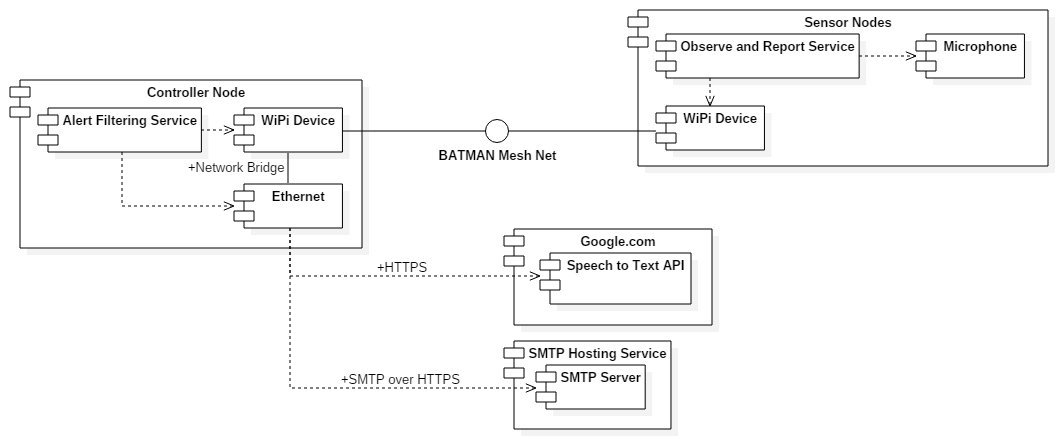
\includegraphics[width=\textwidth, keepaspectratio=true]{Graphics/SystemArchitecture.png}
	\caption{BatSignal system architecture}
\end{figure}

\subsection{System Hardware Architecture}
% In this section, describe the overall system hardware and organization.  Include a list of hardware components (with a brief description of each item) and diagrams showing the connectivity between the components.  If appropriate, use subsections to address each subsystem.
The BatSignal distributed sensor network consists of two types of hardware nodes, consisting primarily of a Raspberry Pi model 2 board. These boards are inexpensive and small computers which will enable the BatSignal network to perform processing and decision making tasks based on input to the system via connected sensors. 

\subsubsection{Control Node}
The BatSignal controller node consists of the Raspberry Pi model 2 board outfitted with a Wi-Pi WLAN module which enables wireless networking capabilities. These nodes also utilize the on board Ethernet adapter to enable a wired network connection to the Internet.

\subsubsection{Sensor Node}
The BatSignal sensor node consists of the Raspberry Pi model 2 board outfitted with a Wi-Pi WLAN module which enables wireless networking capabilities. The sensor nodes are also outfitted with a USB microphone which enables the passive audio recording used to monitor the environment.

\subsection{System Software Architecture}
% In this section, describe the overall system software and organization.  Include a list of software modules (this could include functions, subroutines, or classes), computer languages, and programming computer-aided software engineering tools (with a brief description of the function of each item).  Use structured organization diagrams/object-oriented diagrams that show the various segmentation levels down to the lowest level.  All features on the diagrams should have reference numbers and names.  Include a narrative that expands on and enhances the understanding of the functional breakdown.  If appropriate, use subsections to address each module.
% Note: The diagrams should map to the FRD data flow diagrams, providing the physical process and data flow related to the FRD logical process and data flow.
The system has two types of nodes in the mesh network. The first type of node is a sensor, and the second is the controller node.  There is only one controller node per complete network. The sensor nodes and controller node run different python modules which dictate their behavior. \\\\
Sensor nodes passively wait for input from the attached microphone.  Using Python's speech recognition library the audio input is converted into text.  It is then sent across the mesh network to the controller node. \\\\
The controller node passively waits for input from the sensor nodes. Upon receiving a message it searches the text for alert phrases that are defined in a configuration file and read upon startup. When an alert phrase is identified, an email is composed with the full text of the message and sent to the administrators. The administrators are defined by email address in a configuration file and read upon startup. The controller node is the only node connected directly to the Internet.
% We need to put a specification for the administration console here.


\subsection{Internal Communications Architecture}
% In this section, describe the overall communications within the system; for example, LANs, buses, etc.  Include the communications architecture(s) being implemented, such as X.25, Token Ring, etc.  Provide a diagram depicting the communications path(s) between the system and subsystem modules.  If appropriate, use subsections to address each architecture being employed.
% Note: The diagrams should map to the FRD context diagrams.
The BatSignal distributed sensor network must be capable of communication between nodes, which will be carried out over a wireless mesh network. 

\subsubsection{Wireless Mesh Network}
A mesh network is a topology in which each node connected to the network acts as a relay for data being passed through the network. Data passing through the network may be propagated using either a flooding or a routing technique. Not every node within the network must be connected to every other node on the network. The ability to propagate data by relaying it from node to node allows the network to be both distributed and fault tolerant. The simple fact that the mesh network is being implemented using wireless network adapters makes the mesh network a wireless mesh network. 
\begin{figure}[H]
	\centering
		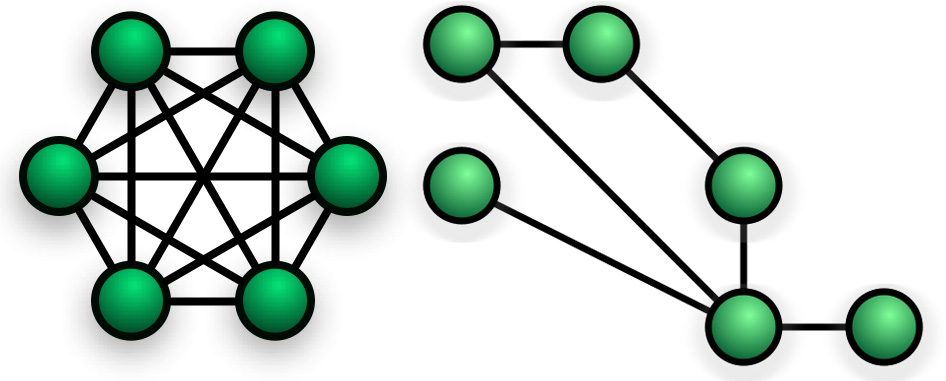
\includegraphics[width=\textwidth, keepaspectratio=true]{Graphics/mesh-networks.jpg}
	\caption{A fully connected, and a partially connected mesh network.}
\end{figure}


\section{Human-Machine Interface}
% This section provides the detailed design of the system and subsystem inputs and outputs relative to the user/operator.  Any additional information may be added to this section and may be organized according to whatever structure best presents the operator input and output designs.  Depending on the particular nature of the project, it may be appropriate to repeat these sections at both the subsystem and design module levels.  Additional information may be added to the subsections if the suggested lists are inadequate to describe the project inputs and outputs.
The BatSignal distributed sensor network is designed to work transparently to the user. The system is designed to passively record audio from the surrounding environment. It does not require any interaction from the user to activate and maintenance can  be performed remotely. Input from administrators to maintain the system is performed through remote access to the controller nodes via ssh and through the administration console. The system outputs email messages upon detecting an alert phrase. Email messages are sent to the list of administrators and contain the full text of the triggering input with the identifier of the node that originally detected the alert phrase.

\subsection{Inputs}
%This section is a description of the input media used by the operator for providing information to the system; show a mapping to the high-level data flows described in Section 1 .2.1, System Overview.  For example, data entry screens, optical character readers, bar scanners, etc.  If appropriate, the input record types, file structures, and database structures provided in Section 3, File and Database Design, may be referenced.  Include data element definitions, or refer to the data dictionary.
%Provide the layout of all input data screens or graphical user interfaces (GUTs) (for example, windows).  Provide a graphic representation of each interface.  Define all data elements associated with each screen or GUI, or reference the data dictionary.
%This section should contain edit criteria for the data elements, including specific values, range of values, mandatory/optional, alphanumeric values, and length.  Also address data entry controls to prevent edit bypassing.
%Discuss the miscellaneous messages associated with operator inputs, including the following:
% •	Copies of form(s) if the input data are keyed or scanned for data entry from printed forms
% •	Description of any access restrictions or security considerations
% •	Each transaction name, code, and definition, if the system is a transaction-based processing system
Input to the system comes in three forms; configuration files, the administration console, and ambient verbal audio. \\\\
Configuration files are read by each node on startup. These files are stored on the controller node in a subdirectory of the installation folder named "config".  The files are stored as "phrases.json" and "admins.json". They each contain a single json object with a list of strings. The list of string for "phrases.json" are the help phrases for the system, each of which is a single English word. The list of strings for "admins.json" are email addresses for the administrators. \\\\
The input to the sensor nodes is through verbal audio signals recorded using the attached microphone.  The controller node receives input in the form of text messages relayed across the mesh network from the sensor nodes. \\\\
The administration console may be used to modify system configuration.

\subsection{Outputs}
% This section describes of the system output design relative to the user/operator; show a mapping to the high-level data flows described in Section 1.2.1.  System outputs include reports, data display screens and GUIs, query results, etc.  The output files are described in Section 3 and may be referenced in this section.  The following should be provided, if appropriate:
% •	Identification of codes and names for reports and data display screens
% •	Description of report and screen contents (provide a graphic representation of each layout and define all data elements associated with the layout or reference the data dictionary)
% •	Description of the purpose of the output, including identification of the primary users
% •	Report distribution requirements, if any (include frequency for periodic reports)
% •	Description of any access restrictions or security considerations
There are three forms of output in the system: internal output from the sensor nodes, email messages to the administrators, and status information available through the administration console. \\\\
The sensor nodes produce text messages containing the converted audio input recorded.  These messages are relayed over the wireless mesh network to the controller node for processing.  The controller node dispatches an email to the administrators containing the plain-text captured input and the node identifier of the sensor which captured the alert. \\\\
% This section requires an elaboration on the administration console and its capabilities for displaying the status of the system.
The administration console displays information concerning the current state of the system.  The state includes sensor node information such as node uptime, node status, and hostnames.  The console will also display any alerts that were emailed.   \\\\

\section{Detailed Design}
% This section provides the information needed for a system development team to actually build and integrate the hardware components, code and integrate the software modules, and interconnect the hardware and software segments into a functional product. Additionally, this section addresses the detailed procedures for combining separate COTS packages into a single system. Every detailed requirement should map back to the FRD, and the mapping should be presented in an update to the RTM and include the RTM as an appendix to this design document.

\subsection{Hardware Detailed Design}
% A hardware component is the lowest level of design granularity in the system.  Depending on the design requirements, there may be one or more components per system.  This section should provide enough detailed information about individual component requirements to correctly build and/or procure all the hardware for the system (or integrate COTS items).
% If there are many components or if the component documentation is extensive, place it in an appendix or reference a separate document.  Add additional diagrams and information, if necessary, to describe each component and its functions, adequately.  Industry-standard component specification practices should be followed.  For COTS procurements, if a specific vendor has been identified, include appropriate item names.  Include the following information in the detailed component designs (as applicable):
% •	Power input requirements for each component
% •	Signal impedances and logic states
% •	Connector specifications (serial/parallel, 11-pin, male/female, etc.)
% •	Memory and/or storage space requirements
% •	Processor requirements (speed and functionality)
% •	Graphical representation depicting the number of hardware items (for example, monitors, printers, servers, I/O devices), and the relative positioning of the components to each other
% •	Cable type(s) and length(s)
% •	User interfaces (buttons, toggle switches, etc.)
% •	Hard drive/floppy drive/CD-ROM requirements
% •	Monitor resolution

\subsubsection{Raspberry Pi 2}
Both versions of BatSignal nodes target the Raspberry Pi model 2 board. These systems have the following capabilities:
\begin{center}
\begin{tabularx}{\textwidth}{ | l | X | }
	\hline
	\multicolumn{2}{ | c | }{\textbf{Raspberry Pi 2 Specifications}} \\
	\hline
	Cost:				& \$35 USD \\
	\hline
	SoC:				& Broadcom BCM2836 \\ 
	\hline
	CPU:				& 900MHz quad-core ARM Cortex-A7 \\
	\hline
	GPU:				& Broadcom VideoCore IV, OpenGL ES 2.0, OpenVG 1080p30 H.264 high-profile encode/decode \\
	\hline
	Memory (SDRAM)iB:	& 1024 MiB \\
	\hline
	USB 2.0 Ports:		& 4 (via intergrated USB hub and LAN9512) \\
	\hline
	Onboard Storage:	& Micro Secure Digital / MicroSD slot \\
	\hline
	Onboard Network:	& 10/100 wired Ethernet RJ45 \\
	\hline
	Real-time Clock:	& None \\
	\hline
	Power Ratings:		& 650 mA, (3.0 W) \\
	\hline
	Power Source: 		& 5 V (DC) via Micro USB type B or GPIO header \\
	\hline
	Size:				& 85.0mm x 56.0 mm x 17mm \\
	\hline
	Weight:				& 40g \\
	\hline
\end{tabularx}
\end{center}

\subsubsection{Wi-Pi WLAN Module}
\begin{center}
\begin{tabularx}{\textwidth}{ | l | X | }
	\hline
	\multicolumn{2}{ | c | }{\textbf{Wi-Pi WLAN Module Specifications}} \\
	\hline
	Cost: 				& \$15.52 \\
	\hline
	Physical Interface: & USB 2.0 \\
	\hline
	Wireless Standards: & IEEE 802.11n \\ 
						& Backward compatible with IEEE 802.11g and IEEE 802.11b \\
	\hline
	Transmission Speed: & 11b: 1/2/5.5/11 Mbps \\
						& 11g: 6/9/12/18/24/36/48/54 Mbps \\
						& 11n: up to 150 Mbps \\
	\hline
	Frequency Range: 	& 2.4 to 2.4835 GHz \\
	\hline
	Working Channel: 	& 1 to 13 \\
	\hline
	Transmit Power: 	& 20dBm (max) \\
	\hline
	Security Features: 	& WPA-PSK/WPA2-PSK \\
						& WPA/WPA2 \\
						& 64/128/152 bit WEP Encryption \\
	\hline
\end{tabularx}
\end{center}

\subsubsection{Microphone}
\begin{center}
\begin{tabularx}{\textwidth}{ | l | X | }
	\hline
	\multicolumn{2}{ | c | }{\textbf{Microphone Specifications}} \\
	\hline
	Frequency Response:		& 50Hz - 18kHz \\
	\hline
	Polar Pattern:		& Directional \\
	\hline
	Resolution:		& 16 Bit/44.1 kHz \\
	\hline
	Sensitivity:	& 56dB @ 1kHz \\
	\hline
	Output Voltage:	&	1.20V \\
	\hline
	Input:	&	USB  \\
	\hline
\end{tabularx}
\end{center}

\subsection{Software Detailed Design}
% A software module is the lowest level of design granularity in the system.  Depending on the software development approach, there may be one or more modules per system.  This section should provide enough detailed information about logic and data necessary to completely write source code for all modules in the system (and/or integrate COTS software programs).
% If there are many modules or if the module documentation is extensive, place it in an appendix or reference a separate document.  Add additional diagrams and information, if necessary, to describe each module, its functionality, and its hierarchy.  Industry-standard module specification practices should be followed.  Include the following information in the detailed module designs:
% •	A narrative description of each module, its function(s), the conditions under which it is used (called or scheduled for execution), its overall processing, logic, interfaces to other modules, interfaces to external systems, security requirements, etc.; explain any algorithms used by the module in detail
% •	For COTS packages, specify any call routines or bridging programs to integrate the package with the system and/or other COTS packages (for example, Dynamic Link Libraries)
% •	Data elements, record structures, and file structures associated with module input and output
% •	Graphical representation of the module processing, logic, flow of control, and algorithms, using an accepted diagramming approach (for example, structure charts, action diagrams, flowcharts, etc.)
% •	Data entry and data output graphics; define or reference associated data elements; if the project is large and complex or if the detailed module designs will be incorporated into a separate document, then it may be appropriate to repeat the screen information in this section
% •	Report layout
There are three separate software components to the BatSignal distributed sensor network.  The sensor nodes, controller node, and administration console. \\\\
The sensor nodes have three python modules installed on them. Two of the modules are from the official python libraries: PyAudio, and SpeechRecognition. These modules are used by the third module: the BatSignal sensor module. The BatSignal sensor module passively listens for input from the microphone. A callback is used to respond when the PyAudio module detects input from the microphone. The callback converts the audio input text using the SpeechRecognition module. The converted text is then logged and sent across the wireless mesh network to the controller node. The sensor network also adjusts for ambient noise.  The system adjusts for ambient noise periodically using the PyAudio module. The time between adjustments is configurable through the administration console. \\\\
The controller node module, upon startup, reads from a series of configuration files stored in a subdirectory of it's installation folder. These configuration files are "phrases.json" and "admins.json", and both are simple JSON files containing a single JSON object and a list of strings. Using python's JSON decoder these files are parsed and stored by the module. The BatSignal control module then switches into a passive listening mode from which it waits for messages from the sensor nodes. Upon receiving a message from a sensor node it parses the JSON of the message into its components. The JSON message contains the identifier of the dispatching sensor node, the time the message was sent, and the contents of the message. The contents of the message are parsed using a simple string comparison method. The string is split using the delimiters of whitespace and control characters (commas, periods, etc.). Each word in the split string is then compared to every alert phrase from "prases.json"  Upon finding a match an email is composed containing the name of the sensor node the message originated from, the time the audio was recorded, and the full contents of the audio converted to text. The email is then mailed to all addresses listed in "admins.json".  \\\\
% This section requires an elaboration on the design and implementation of the administration console.
The administration console will be the central configuration point for the BatSignal network.The backend for the console will be written using the python library Flask.  The administration console will allow for the modification of the "phrases.json" and "admins.json" configuration files and will contain information related to the current BatSignal deployment.  It will have the capability of performing diagnostic tasks as well as displaying current deployment information.  These diagnostic tasks include restarting nodes, changing hostnames, and testing connectivity to all nodes.  Deployment information that will be seen within the console includes hostnames, assigned IP addresses, and sensor status.  The console will contain a panel that will detail the same alerts that have been emailed, and will be updated in real-time.  Any nonfunctioning sensors will be visible within this panel.      \\\\ 

\end{document}